\documentclass[12pt]{article}

\usepackage{polski}
\usepackage[utf8]{inputenc}
\usepackage[T1]{fontenc}
%\usepackage{indentfirst}
\usepackage{amsfonts}
\usepackage{graphicx}
\usepackage{caption}
\usepackage{multirow}
\usepackage{booktabs}
\usepackage{amssymb}
\usepackage[top=2cm, bottom=2cm, left=3cm, right=3cm]{geometry}
\usepackage{mathrsfs}
\usepackage{tikz}
\usepackage{pgfplots}
%\pagestyle{empty}
\usepackage{listings}
\usepackage{titlesec}
\usepackage{hyperref}
\usepackage{graphicx}
\usepackage{subfig}
\usepackage{natbib}
\usepackage{rotating}
\usepackage{float}
\usepackage{pdfpages}
\usepackage{pdflscape}
\usepackage{listings}

\title{\textbf{Sprawozdanie - Stacja do wykrywania wyładować atmosferycznych}\\KNEKSA}
\author{Michał Wieczorek {226284}\\ Mateusz Otto {226312}}
\date{\today}

\begin{document}
\maketitle
\newpage
\section{Opis projektu}
Celem projektu jest konstrukcja niskobudżetowego uniwersalnego odbiornika fal krótkich o zakresie częstotliwości 3 kHz - 300 kHz. Wyładowanie atmosferyczne generuje fale elektromagnetyczne w bardzo szerokim zakresie częstotliwości. Są to impulsy, które mogą zostać odebrane ponad 1000 km od wystąpienia wyładowania. Szczegółowy teoretyczny opis zjawiska można znaleźć np. na Wikipedii. Dla częstotliwości niższych niż 100 kHz impulsy wyraźnie wybijają się ponad szum atmosferyczny, co pozwala z łatwością odebrać sygnał. Odbiornik będzie posiadać dwa wejścia na anteny ferrytowe typu H-field, co pozwoli określić przybliżoną odległość i kierunek odebranego sygnału. Anteny zostaną skonstruowane przez wykonawców projektu, ich parametry zostaną eksperymentalnie wyznaczone. Po pomyślnym zainstalowaniu odbiornika następnym krokiem będzie konstrukcja kilku następnych, co pozwoli na dokładniejsze określenie lokalizacji wystąpienia wyładowania za pomocą porównań czasów odebrania sygnału (Time of arrival method). Dane z odbiornika będą przesyłane na serwer w celu ich analizy. Projekt zakłada ukończenie prac nad jednym odbiornikiem i uruchomienie go przed końcem roku 2017. Jednym z założeń jest łatwe wprowadzanie zmian i dodatkowych modułów do odbiornika tak, aby jego użytkownicy mogli dalej go rozwijać oraz mieli możliwość prowadzenia badań. Planowane jest udostępnienie ukończonej stacji do użytku jako projekt wykonany w kole naukowym.

\section{Zrealizowane zadania i przeprowadzone testy}
\subsection{Schemat prototypu układu filtrów i wzmacniaczy skonstruowany w programie LTSpice}
\begin{figure}[H]
\begin{center}
\includegraphics[width=1\textwidth]{figures/schemat1.png}
\caption{I część Schematu układu}
\end{center}
\end{figure}
\begin{figure}[H]
\begin{center}
\includegraphics[width=1\textwidth]{figures/schemat2.png}
\caption{II część Schematu układu}
\end{center}
\end{figure}
\begin{figure}[H]
\begin{center}
\includegraphics[width=1\textwidth]{figures/ampl_faz.png}
\caption{Charakterystyka Bodego układu}
\end{center}
\end{figure}

\subsection{Skonstruowanie prototypu układu}
\begin{figure}[H]
\begin{center}
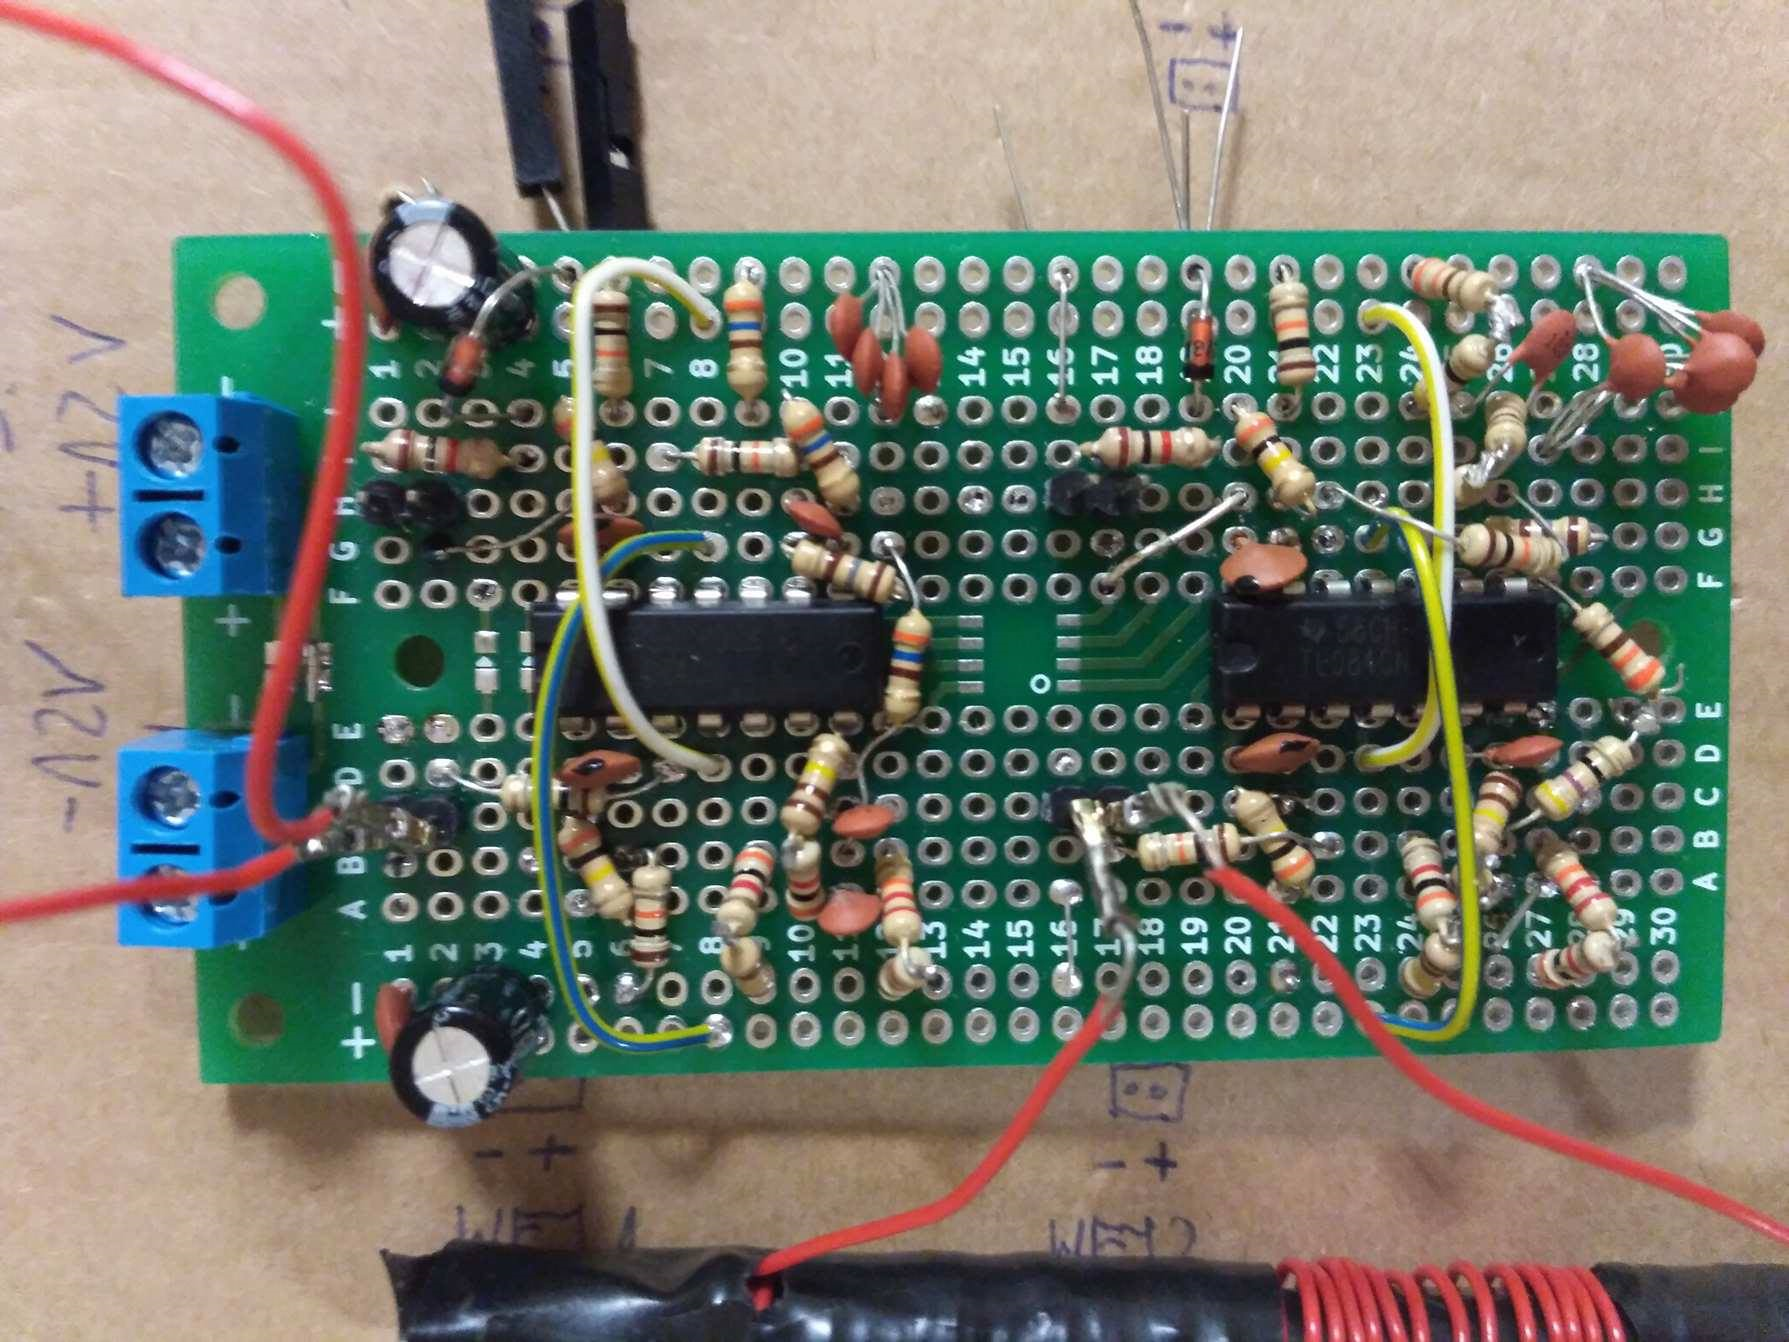
\includegraphics[width=0.95\textwidth]{figures/plytka.png}
\caption{Prototyp układu}
\end{center}
\end{figure}

\subsection{Skonstruowanie anten kierunkowych}
\begin{figure}[H]
\begin{center}
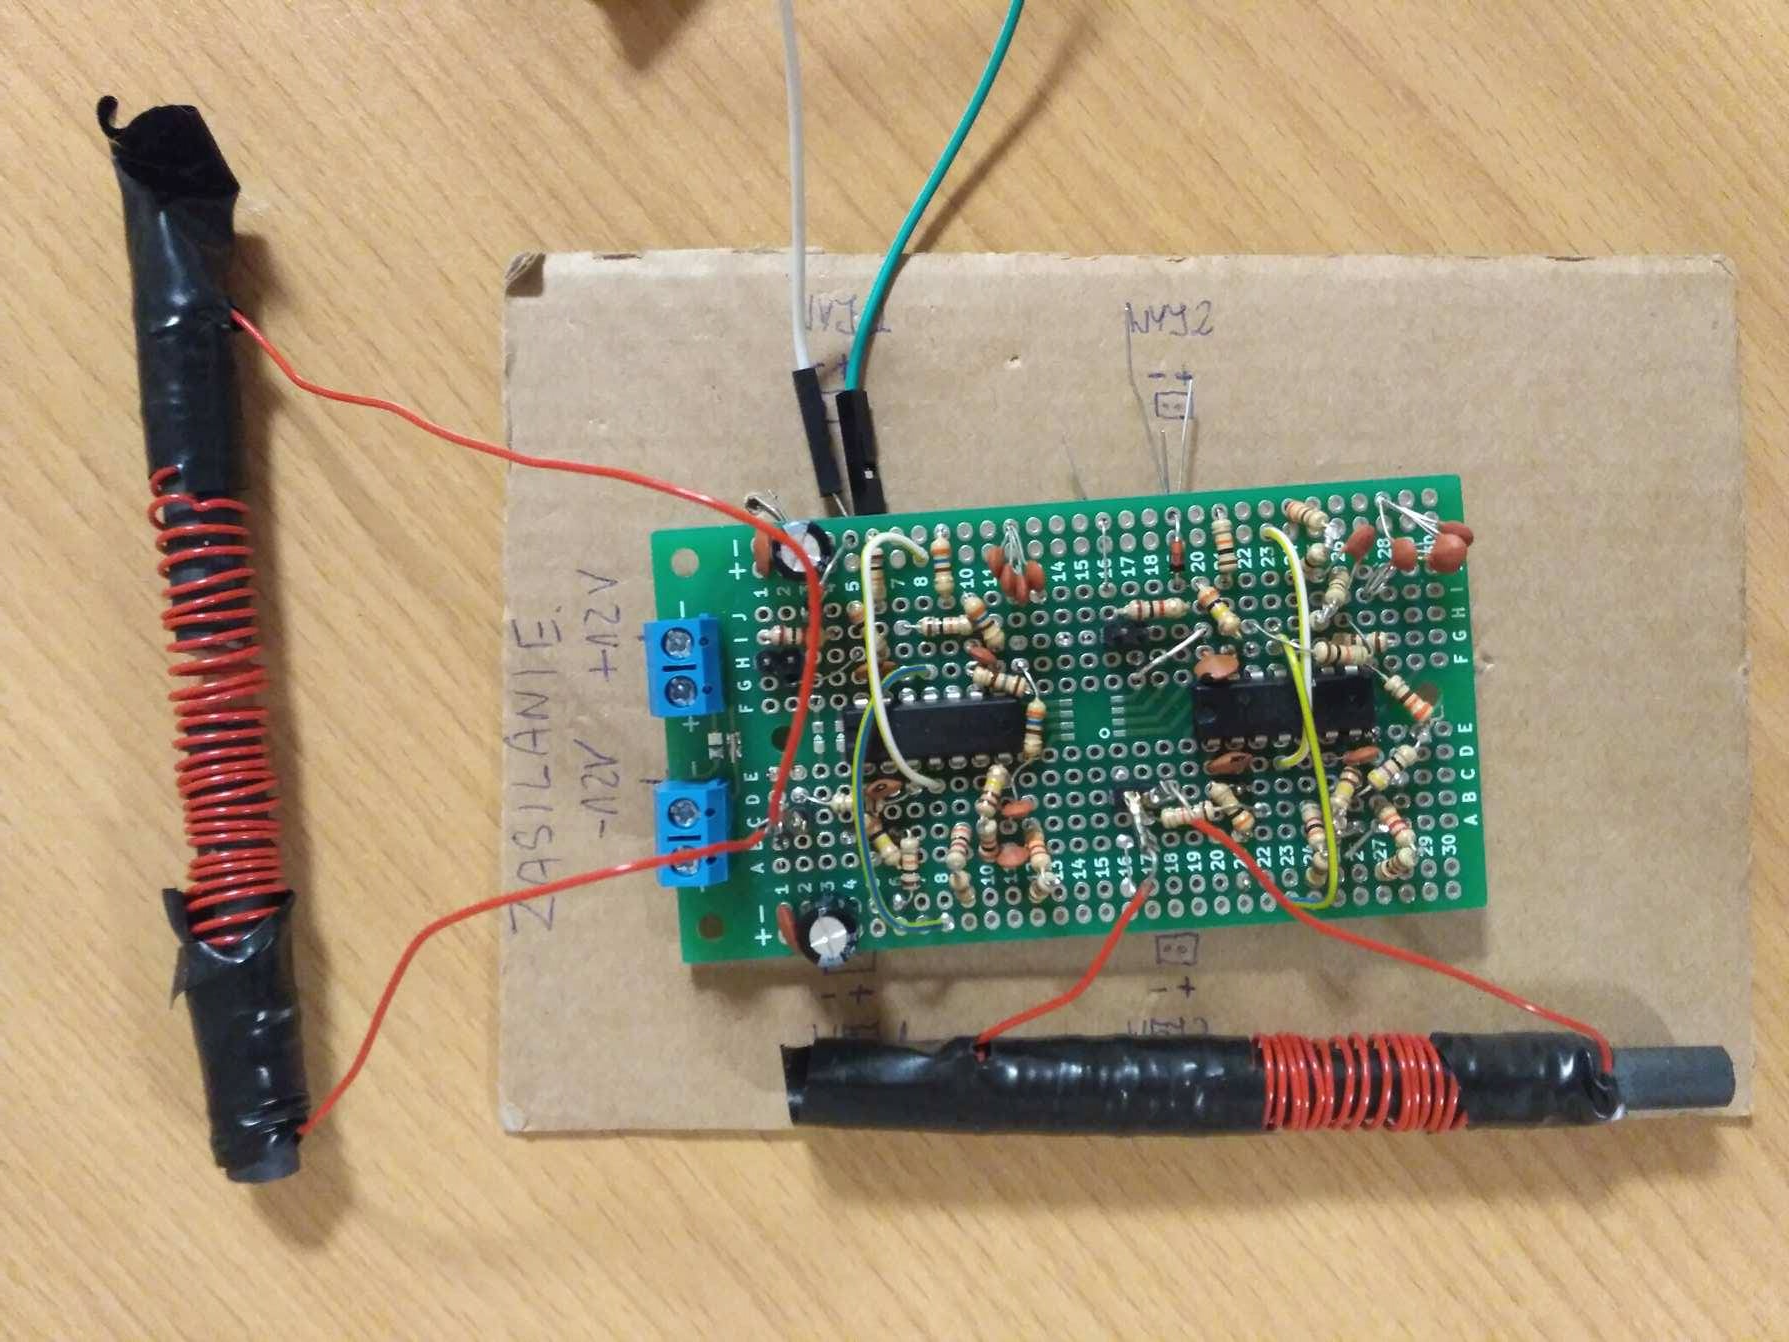
\includegraphics[width=0.95\textwidth]{figures/ukladantena.png}
\caption{Anteny kierunkowe ułożone pod kątem prostym podłączone do prototypu układu}
\end{center}
\end{figure}

\subsection{Testy układu z wyjściem podłączonym do oscyloskopu}
\begin{figure}[H]
\begin{center}
\includegraphics[width=0.95\textwidth]{figures/oscyloskop.png}
\caption{Wykrycie wyładowania atmosferycznego przez układ}
\end{center}
\end{figure}

\subsection{Próbkowanie sygnału analogowego za pomocą mikrokontrolera STM32 Nucleo}
\begin{figure}[H]
\begin{center}
\includegraphics[width=0.95\textwidth]{figures/uklad.png}
\caption{Zmontowany układ}
\end{center}
\end{figure}
\begin{figure}[H]
\begin{center}
\includegraphics[width=0.95\textwidth]{figures/stm.png}
\caption{STMStudio - obserwacja sygnału na wyjściu układu}
\end{center}
\end{figure}
%\begin{landscape}
%\centering
%\includepdf[angle=90]{figures/schematcal.pdf}
%\end{landscape}

\newpage

\subsection{Próbkowanie i przesyłanie sygnału}
Za pomocą STM32CubeMX, graficznego interfejsu do konfiguracji peryferiów układu i biblioteki HAL sygnał odebrany z anteny i próbkowany za pomocą przetwornika ADC jest przypisywany do bufora bez użycia zasobów procesora za pomocą Direct Memory Acces, co oznacza bezpośredni dostęp do pamięci, umożliwiający wysyłanie danych bez udziału procesora w transferze danych. Następnie, dane analogicznie pobierane są z bufora i przesyłane do interfejsu UART. Konwerter USB-UART FTDI jest wbudowany na płytce STM Nucleo i pozwala na przesłanie danych do komputera za pomocą kabla USB.\\
\\Aby uzyskać większą częstotliwość na zegarze pętli głównej PLL dołączono dodatkowy kwarc o częstotliwości taktowania 8MHz (seryjnie znajduje się on na płytce). Zewnętrzny kwarc zmniejsza również błąd wewnętrznego timera procesora. Wejście ADC podpięto pod pin PA0, z kolei interfejs UART pod piny PA2, PA3 zgodnie ze schematem wyprowadzeń w specyfikacji płytki nucleo. 

\begin{figure}[H]
\begin{center}
\includegraphics[width=1\textwidth]{figures/cube.png}
\caption{Konfiguracja pinów w programie STM32CUBEMX}
\end{center}
\end{figure}

\newpage

W pętli głównej ustawiono maksymalną częstotliowość - 100MHz, z kolei do perypetii (APB1) dociera połowa tej wielkości czyli 50MHz. W lewym dolnym rogu wybieramy częstotliwość taktowania kwarcu zewnętrznego oraz przesuwamy znacznik na HSE aby z niego skorzystać.

\begin{figure}[H]
\begin{center}
\includegraphics[width=1\textwidth]{figures/zegar.png}
\caption{Konfiguracja zegara}
\end{center}
\end{figure}

\begin{figure}[H]
    \centering
    \subfloat[Konfiguracja ADC]{{\includegraphics[width=0.45\textwidth]{figures/adc.png} }}
    \qquad
    \subfloat[Konfiguracja UART]{{\includegraphics[width=0.45\textwidth]{figures/uart.png} }}
    \caption{Ustawienie podstawowych parametrów interfejsów}%
    \label{fig:example}%
\end{figure}

\newpage

\lstset{language=C++,
                basicstyle=\ttfamily,
                keywordstyle=\color{blue}\ttfamily,
                stringstyle=\color{red}\ttfamily,
                commentstyle=\color{green}\ttfamily,
                morecomment=[l][\color{magenta}]{\#}
}

\begin{lstlisting}
/* Includes ---------------------------------------------*/
#include "main.h"
#include "stm32f4xx_hal.h"

/* Private variables ------------------------------------*/
ADC_HandleTypeDef hadc1;
DMA_HandleTypeDef hdma_adc1;
UART_HandleTypeDef huart2;
DMA_HandleTypeDef hdma_usart2_tx;
uint8_t buffor[8]; /* 8-bitowy bufor na zczytana wartosc */
uint16_t length;   /* rozmiar bufora */

/* Private function prototypes --------------------------*/
void SystemClock_Config(void);
static void MX_GPIO_Init(void);
static void MX_DMA_Init(void);
static void MX_ADC1_Init(void);
static void MX_USART2_UART_Init(void);

int main(void)
{
  /* Reset of all peripherals, Initializes 
  the Flash interface and the Systick. */
  HAL_Init();
  /* Configure the system clock */
  SystemClock_Config();
  /* Initialize all configured peripherals */
  MX_GPIO_Init();
  MX_DMA_Init();
  MX_ADC1_Init();
  MX_USART2_UART_Init();
  
  /* pobranie rozmiaru bufora */
  length = sizeof(buffor); 
  /* rozpoczecie dzialania adc */
  HAL_ADC_Start_DMA(&hadc1, (uint32_t*)buffor, length);
  /* uruchomienie wysylania uart*/
  HAL_UART_Transmit_DMA(&huart2, buffor, length);

  /* Infinite loop */
  while (1){}
}
\end{lstlisting}

\newpage

\subsection{Odbiór i analiza danych}
Do odbioru i analizy danych wykorzystano program Labview. Dane są przekazywane do wirtualnego portu w komputerze i odczytywane w programie. Sygnał można obejrzeć na generowanym na bieżąco wykresie, a kiedy wykryty zostanie impuls, próbki wraz z czasem wystąpienia impulsu zostają zapisywane do pliku.

\begin{figure}[H]
\begin{center}
\includegraphics[width=1\textwidth]{figures/labview1.png}
\caption{Schemat blokowy w programie Labview}
\end{center}
\end{figure}

\begin{figure}[H]
\begin{center}
\includegraphics[width=1\textwidth]{figures/labview2.png}
\caption{Przebieg sygnału odbieranego przez antenę oglądany w Labview}
\end{center}
\end{figure}

\end{document}